%Sample usage of usuthesis.cls
\documentclass[cs, msthesis]{usuthesis}

%{{{ Some useful packages, modify as needed
\usepackage{epsfig}
\usepackage{amssymb}           % add ams symbols stuff
\usepackage{caption}		% needed for listing captions
\usepackage{graphicx}          	% add graphics
\usepackage{subfigure}
\usepackage{color}             	% grants control of link text colors.
\usepackage{algorithm2e}
\usepackage{listings}		% code listings
\usepackage{pdflscape}
\usepackage{hyperref}          	% make contents/ref/citations clickable
\usepackage{epstopdf}
\usepackage{color}
\usepackage{enumerate}		% lists of items
\usepackage{url} 			% url in bib
%}}}

% for formatting code
\lstset{
	language=C++,                		% choose the language of the code
	basicstyle=\footnotesize,       		% the size of the fonts that are used for the code
	numbers=left,                   		% where to put the line-numbers
	numberstyle=\footnotesize,		% the size of the fonts that are used for the line-numbers
	stepnumber=1,                   		% the step between two line-numbers. If it is 1 each line will be numbered
	firstnumber=100,
	lineskip={5pt},
	aboveskip={2\baselineskip},
	belowskip={0\baselineskip},
	xleftmargin=0mm,				% left margin of listing section
	floatplacement=t,
	numbersep=-15pt,                  	% how far the line-numbers are from the code
	backgroundcolor=\color{white},  	% choose the background color. You must add \usepackage{color}
	showspaces=false,               		% show spaces adding particular underscores
	showstringspaces=false,         	% underline spaces within strings
	showtabs=false,                 		% show tabs within strings adding particular underscores
	frame=tb,           				% adds a frame around the code
	tabsize=4,          				% sets default tabsize to 2 spaces
	captionpos=b,           			% sets the caption-position to bottom
	breaklines=true,        			% sets automatic line breaking
	breakatwhitespace=false,    		% sets if automatic breaks should only happen at whitespace
	numberbychapter=true,
	escapeinside={\%*}{*)}          		% if you want to add a comment within your code
}
\lstloadlanguages{
	C++
 }

\intextsep=10mm					% controls spacing before and after figures and tables
\belowcaptionskip=-5mm

%Set all linked content to be plain black text
\hypersetup{
	colorlinks,%
	citecolor=black,%
	filecolor=black,%
	linkcolor=black,%
	urlcolor=black
}


% Author and Title Information
\author{Jesse Victors}
\title{EsgalDNS: \\ Namecoin-based Anonymous Domain Name Service \\ for Tor Hidden Services}


% The Committee
\majorprof{Dr. Ming Li}
\firstreader{Dr. Nicholas Flann}
\secondreader{Dr. Daniel Watson}


% Graduate Dean, Update as necessary
\graddean{Dr. Mark R. McLellan} 
\deantitle{Vice President for Research and}
\deansecondtitle{Dean of the School of Graduate Studies}

% Degree Information
\degree{Master of Science}
\month{May}
\year{2014}

\begin{document}

	%{{{ Frontmatter
	\preliminaries   % set frontmatter style

	\maketitle
	\makecopyright        % optional

	

\begin{abstract}
% A space is needed before the text starts so that the first paragraph
% is indented properly.

The Tor network is a second-generation onion routing system that aims to provide anonymity, privacy, and Internet censorship resistance to its users. In recent years it has grown significantly in response to revelations of national and global electronic surveillance, and remains one of the most popular and secure anonymity network in use today. Tor is also known for its support of anonymous websites within its network. Decentralized and secure, the domain names for these services are tied to public key infrastructure (PKI) but are challenged by their long and technical addresses. In response to this difficulty, in this thesis I introduce a novel and decentralized Tor-powered DNS system that provides unique and human-meaningful domain names to Tor hidden services.

\end{abstract}

	\begin{publicabstract}
\centerline{CHAD M. MAUGHAN}
\vspace{12pt}
%Leave a blank line for formatting

Rich Web Applications (RWA) that are data driven and feature responsive user interfaces are rapidly growing in popularity.  Popular sites such as Twitter, Pandora, and Angry Birds (browser version) are all examples of popular RWAs.  These RWAs are more complex and are developed differently than many previous web sites.  More of the processing power needed to run these applications is performed on the client machine, not the server.  Due to this development strategy, testing tools need new techniques to identify web application variables, capture errors, and identify problems.  In this thesis, I introduce novel techniques to identify variables in RWA semantic URLs and automatically generate tests for RWAs using a form of testing called combinatorial testing.

\end{publicabstract}

	%

\begin{dedication}

This work is dedicated to the developers and community behind the Tor Project and the Tails OS. These individuals work tirelessly to preserve the privacy and security of everyday citizens, journalists, activists, and others around the globe, providing the much-needed service of private conversations in a very public world.

\end{dedication}
  % optional
	%
%https://tex.stackexchange.com/questions/656/how-to-create-acknowledgements-in-the-report-class
\begin{dedication}

I would like to thank my major professor, Dr. Ming Li, for his continual guidance. His analysis, suggestions, and descriptions of possible attacks were instrumental in developing and solidifying this work. I would also like to extend thanks for the rest of my committee: Dr. Dan Watson and Dr. Nick Flann for their support. 

I would also like to thank Tor developers Mark Ellzey, Yawning Angel, and Nick Mathewson for their assistance with libevent and Tor technical support, Sarbajit Mukherjee for his commentary and suggestions on this work, and the Tor community for their continued support of OnioNS.

\end{dedication}     % optional

	\tableofcontents
	\listoftables
	\listoffigures

	%    \include{doc/notation}  % optional
	%    \include{doc/acronyms}  % optional
	%}}}
	%{{{ The main body of the thesis
	\body  % set main body style

	% Chapters
	
\chapter{INTRODUCTION}

\section{Onion Routing}

As the prevalence of the Internet and other communication has grown, so too has the development and usage of privacy-enhancing systems. These are tools and protocols that provide privacy by obfuscating the link between a user's identification or location and their communications. Privacy is not achieved in traditional Internet connections because SSL/TLS encryption cannot hide IP and TCP headers, which must be exposed to allow routing between two parties; eavesdroppers can easily break user privacy by monitoring these headers. A closely related property is anonymity -- a part of privacy where user activities cannot be tracked and their communications are indistinguishable from others. Tools that provide these systems hold a user's identity in confidence, and privacy and anonymity are often provided together. Following a general distrust of unsecured Internet communications and in light of the 2013-current revelations by Edward Snowden of Internet mass-surveillance by the NSA, GCHQ, and other members of the Five Eyes, users have increasingly turned to these tools for their own protection. Privacy-enhancing and anonymity tools may also be used by the military, researchers working in sensitive topics, journalists, law enforcement running tip lines, activists and whistleblowers, or individuals in countries with Internet censorship. These users may turn to proxies or VPNs, but these tools often track their users for liability reasons and thus rarely provide anonymity. Furthermore, they can easily voluntarily or be forced to break confidence to destroy user privacy. More complex tools are needed for a stronger guarantee of privacy and anonymity.

Today, most anonymity tools descend from mixnets, an early anonymity system invented by David Chaum in 1981.\cite{chaum2003untraceable} In a mixnet, user messages are transmitted to one or more mixes, who each partially decrypt, scramble, delay, and retransmit the messages to other mixes or to the final destination. This enhances privacy by heavily obscuring the correlation between the origin, destination, and contents of the messages. Mixnets have inspired the development of many varied mixnet-like protocols and have generated significant literature within the field of network security.\cite{edman2009anonymity}\cite{syverson2011peel}

Mixnet descendants can generally be classified into two distinct categories: high-latency and low-latency systems. High-latency networks typically delay traffic packets and are notable for their greater resistance to global adversaries who monitor communication entering and exiting the network. However, high-latency networks, due to their slow speed, are typically not suitable for common Internet activities such as web browsing, instant messaging, or the prompt transmission of email. Low-latency networks, by contrast, do not delay packets and are thus more suited for these activities, but they are more vulnerable to timing attacks from global adversaries.\cite{dingledine2004tor} In this work, we detail and introduce new functionality within low-latency protocols.

Onion routing is a technique for enhancing privacy of TCP-based communication across a network and is the most popular low-latency descendant of mixnets in use today. It was first designed by the U.S. Naval Research Laboratory in 1997 for military applications\cite{syverson1997anonymous}\cite{reed1998anonymous} but has since seen widespread usage. In onion routing with public key infrastructure (PKI), a user selects a set network nodes, typically called \emph{onion routers} and together a \emph{circuit}, and encrypts the message with the public key of each router. Each encryption layer contains the next destination for the message -- the last layer contains the message's final destination. As the \emph{cell} containing the message travels through the network, each of these onion routers in turn decrypt their encryption layer like an onion, exposing their share of the routing information. The final recipient receives the message from the last router, but is never exposed to the message's source.\cite{syverson2011peel} The sender therefore has privacy because the recipient does not know the sender's location, and the sender has anonymity if no identifiable or distinguishing information is included in their message.

\begin{figure}[htbp]
	\centering
	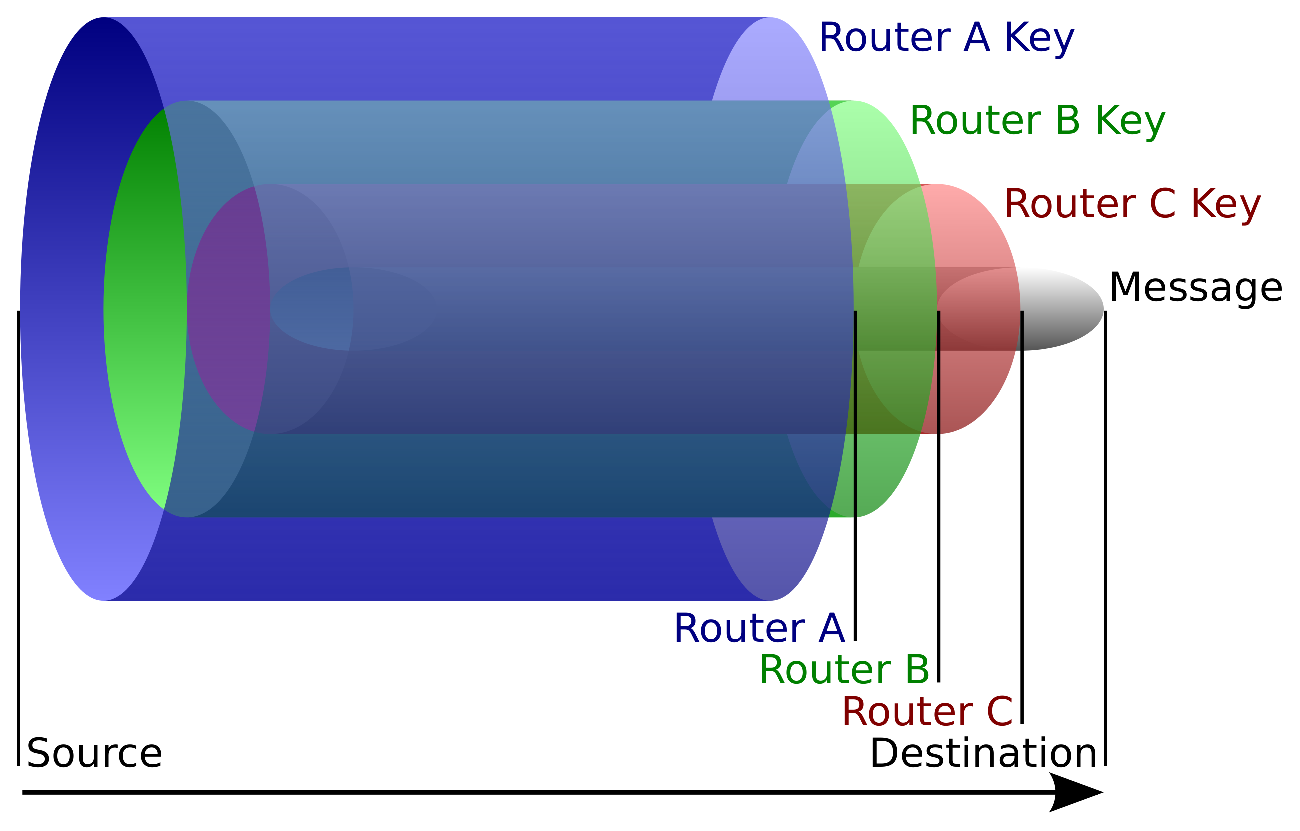
\includegraphics[width=0.5\textwidth]{images/onion-diagram.eps}
	\caption{An example cell and message encryption in an onion routing scheme. Each router ``peals'' off its respective layer of encryption; the final router exposes the final destination.}
\end{figure}

The first generation of onion routing used circuits fixed to a length of five, assumed a static network topology, and most notably, introduced the ability to mate two circuits at a common router or server. This last capability enabled broader anonymity where the circuit users were anonymous to each other and to the common server, a capability that was adopted and refined by later generation onion routers. Second generation introduced variable-length circuits, multiplexing of all user traffic over circuits, exit policies for the final router, and assumed a dynamic network by routing updates throughout the network. A client, Alice, in second-generation onion routers also distributed symmetric keys through the cell layers. If routers remember the destinations for each message they received, the recipient Bob can send his reply backwards through the circuit and each router re-encrypts the reply with their symmetric key. Alice unwraps all the layers, exposing the Bob's reply. The transition from public-key cryptography to symmetric-key encryption significantly reduced the CPU load on onion routers and enabled them to transfer more packets in the same amount of time. However, while influential, first and second generation onion routing networks have fallen out of use in favor of third-generation systems.\cite{syverson2011peel}

\section{Tor}

Tor is a third-generation onion routing system. It was invented in 2002 by Roger Dingledine, Nick Mathewson, and Paul Syverson of the Free Haven Project and the U.S. Naval Research Laboratory\cite{dingledine2004tor} and is the most popular onion router in use today. Tor inherited many of the concepts pioneered by earlier onion routers and implemented several key changes:\cite{syverson2011peel}\cite{dingledine2004tor}

\begin{itemize}
	\item \textbf{Perfect forward secrecy:} Rather than distributing keys via onion layers, Tor clients negotiate ephemeral symmetric encryption keys with each of the routers in turn, extending the circuit one router at a time. These keys are then purged when the circuit is torn down; this achieves perfect forward secrecy, a property that ensures that the session encryption keys will not be revealed if long-term public keys are later compromised.
	\item \textbf{Circuit isolation:} Second-generation onion routers mixed cells from different circuits in realtime, but later research could not justify this as an effective defence against an active adversary.\cite{syverson2011peel} Tor abandoned this in favor of isolating circuits from each other inside the network, although it recycles TCP/IP links between routers.
	\item \textbf{Three-hop circuits:} Previous onion routers used long circuits to provide heavy traffic mixing. Tor removed mixing and fell back to using short circuits of minimal length. With three relays involved in each circuit, the first router (the \emph{guard}) is exposed to the user's IP address. The middle router passes onion cells between the guard and the final router (the \emph{exit}) and its encryption layer exposes it to neither the user's IP nor its traffic. The exit processes user traffic, but is unaware of the origin of the requests. While the choice of middle and exits can be routers can be safely random, the guard must be chosen once and then consistently used to avoid a large cumulative chance of leaking the user's IP to an attacker. This is of particular importance for circuits from hidden services.\cite{bauer2007low}\cite{overlier2006locating}
	\item \textbf{Standardized to SOCKS proxy:} Tor simplified the multiplexing pipeline by transitioning from application-level proxies (HTTP, FTP, email, etc) to a TCP-level SOCKS proxy, which multiplexed user traffic and DNS requests through the onion circuit regardless of any higher protocol. The disadvantage to this approach is that Tor's client software has less capability to cache data and strip identifiable information out of a protocol. The countermeasure was the Tor Browser, a fork of Mozilla's open-source Firefox with a focus on security and privacy. To reduce the risks of users breaking their privacy through Javascript, it ships with the NoScript extension which blocks all web scripts not explicitly whitelisted. The browser also forces all web traffic, including DNS requests, through the Tor SOCKS proxy, provides a Windows-Firefox user agent regardless of the native platform, and includes many sanitization, security, and privacy enhancements not included in native Firefox. The browser also utilizes the Electronic Frontier Foundation's HTTPS Everywhere extension to re-write HTTP web requests into HTTPS whenever possible, providing an additional encryption layer that hides web traffic from exit routers.
	\item \textbf{Directory servers:} Tor introduced a set of trusted directory servers, called directory authorities, to collect, digitally sign, and distribute network information such as the IP addresses and public keys of onion routers. Onion routers mirror the network information from the directories, distributing the bandwidth load. This simplified approach is more flexible and scales faster than the previous flooding approach, but relies on the trust of central directory authorities. Tor ensures that each authority is independently maintained in multiple locations and jurisdictions, reducing the likelihood of an attacker compromising all of them.\cite{syverson2011peel} We describe the contents and format of this network information in section \ref{sec:ConsensusDocs}.
	\item \textbf{Dynamic rendezvous with hidden services:} In previous onion routers, circuits mated at a fixed common node and did not use perfect forward secrecy. Tor introduced a distributed hashtable to record the location of the introduction node for a given hidden service. Following the initial handshake, the server and the client then meet at a different onion router chosen by the client. This approach significantly increased the reliability of hidden services and distributed the communication load across multiple rendezvous points.\cite{dingledine2004tor} We provide additional details on the hidden service protocol in section \ref{sec:HiddenServices} and our motivation for addition infrastructure in section \ref{sec:Motivation}.
\end{itemize}

As of March 2015, Tor has 2.3 million daily users that together generate 65 Gbit/s of traffic. Tor's network consists of nine directory authorities and 6,600 onion routers in 83 countries.\cite{TorMetrics} In a 2012 Top Secret U.S. National Security Agency presentation leaked by Edward Snowden, Tor was recognized as the "the king of high secure, low latency Internet anonymity".\cite{landau2014highlights}\cite{plak2014anonymous} In 2014, BusinessWeek claimed that Tor was ``perhaps the most effective means of defeating the online surveillance efforts of intelligence agencies around the world.''\cite{TorBusinessWeek}

\subsection{Design}

Tor's design focuses on being easily deployable, flexible, and well-understood. Tor also places emphasis on usability in order to attract more users; more user activity translates to an increased difficulty of isolating and breaking the privacy of any single individual. Tor however does not manipulate any application-level protocols nor does it make any attempt to defend against global attackers. Instead, its threat model assumes that the capabilities of adversaries are limited to observing fractions of Tor traffic, that they can actively delay, delete, or manipulate traffic, that they may attempt to digitally fingerprint packets, that they may run onion routers themselves, and that they may compromise a fraction of other existing routers. Together, most of the assumptions may be broadly classified as traffic analysis attacks. Tor's final focus is defending against these types of attacks.\cite{dingledine2004tor}

\subsection{Circuit Construction}

\begin{figure}[htdp]
	\begin{minipage}[b]{0.48\linewidth}
		\centering
		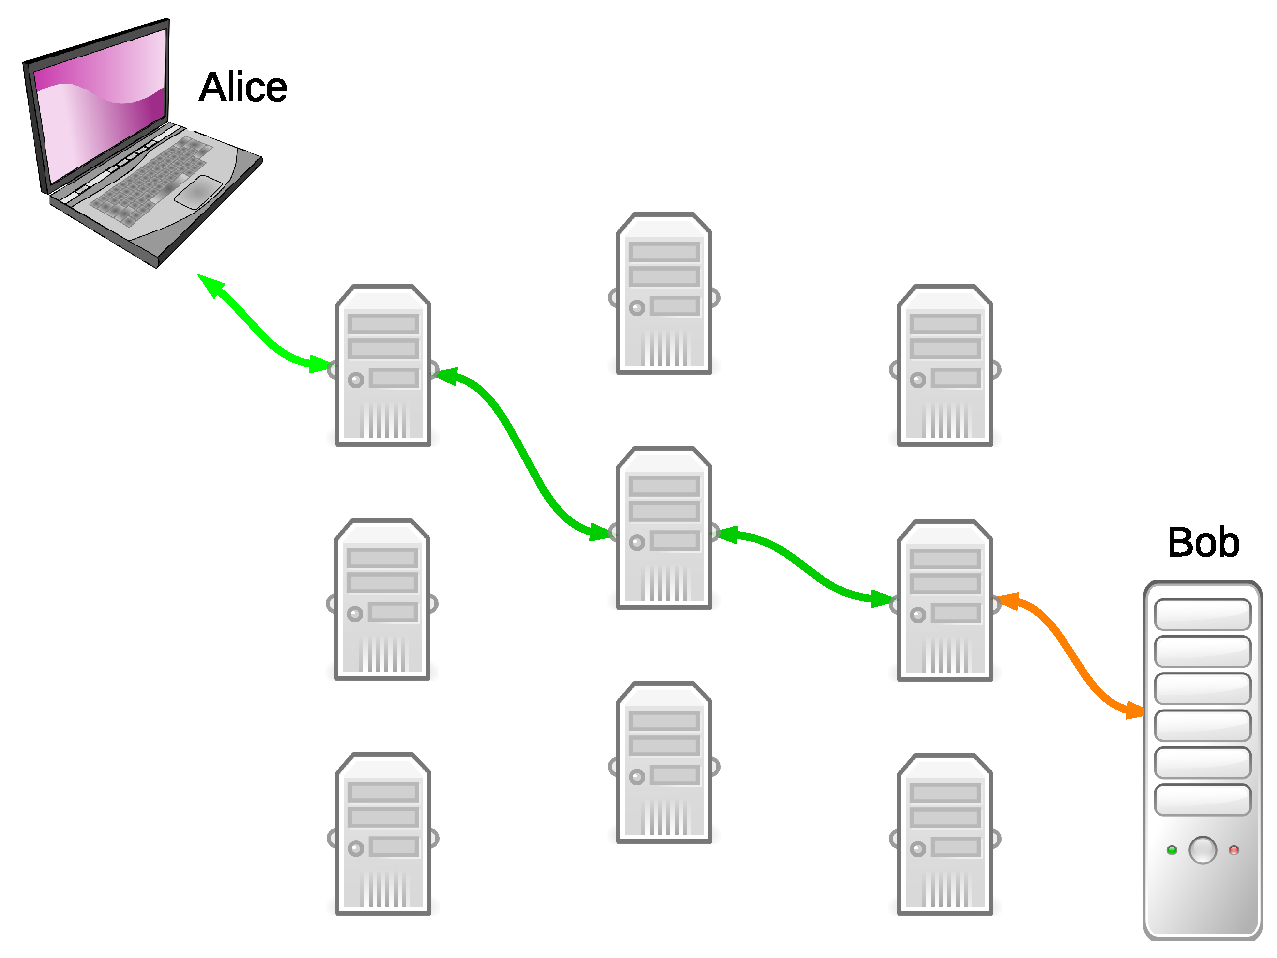
\includegraphics[width=\textwidth]{images/LucidCharts/Tor_Circuit_Orig.pdf}
	\end{minipage}
	\hspace{0.5cm}
	\begin{minipage}[b]{0.48\linewidth}
		\centering
		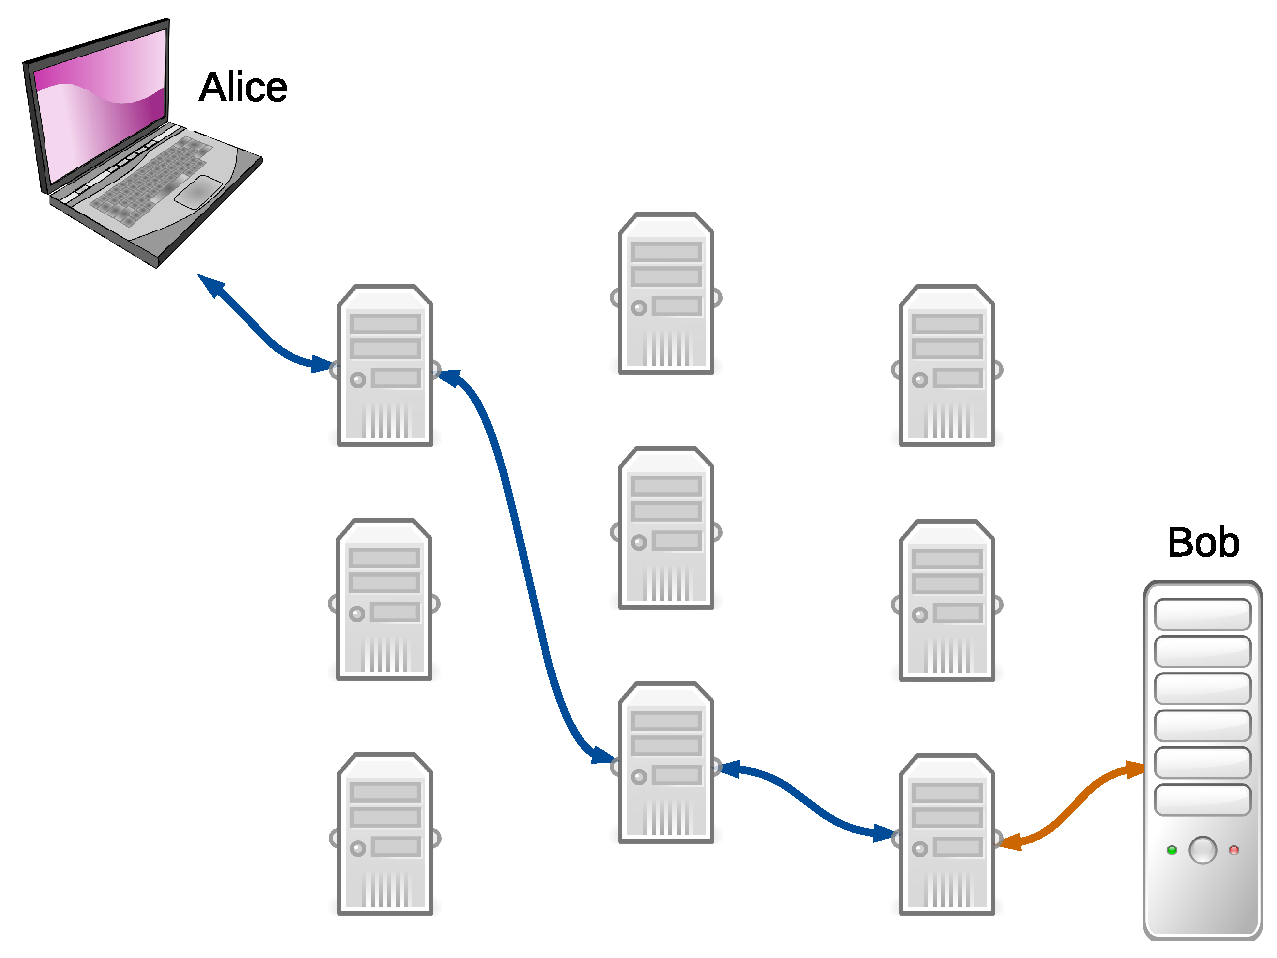
\includegraphics[width=\textwidth]{images/LucidCharts/Tor_Circuit_Change.pdf}
	\end{minipage}
	\caption{Alice communicates privately to Bob through a Tor circuit. Her communication path consists of three routers, an entry, middle, and exit. Although Bob's identity and location is known to Alice, the Tor circuit prevents Bob from knowing Alice's identity or location. At a later time, Alice may construct a different circuit to Bob, giving her a new identity from Bob's perspective. Each encrypted Tor link is shown in green, the final connection from the exit to Bob, shown in orange, is optionally encrypted.}
	\label{fig:torOverview}
\end{figure}

\subsubsection{Overview}

Let Alice be a client who wishes to enhance her privacy by using Tor but does not run a Tor router herself. Her basic procedure for initializing her own circuit is as follows:

\begin{enumerate}
	\item Alice selects a Tor router $ R_{1} $ and sets up an authenticated encrypted connection to it.
	\item Alice selects a second router $ R_{2} $ and tells $ R_{1} $ to build a TCP link to it. 
	\item Alice uses her $ R_{1} $ tunnel to establish an authenticated encrypted connection with $ R_{2} $.
	\item Alice selects an $ R_{3} $ and uses the $ Alice \leftrightarrow R_{1} \leftrightarrow R_{2} $ tunnel to tell $ R_{2} $ to connect to $ R_{3} $.
	\item Alice establishes an authenticates encrypted connection with $ R_{3} $ over the \\ $ Alice \leftrightarrow R_{1} \leftrightarrow R_{2} $ tunnel.
\end{enumerate}

Following the successful circuit construction, she can then send messages out of $ R_{3} $ through the $ Alice \leftrightarrow R_{1} \leftrightarrow R_{2} \leftrightarrow R_{3} $ tunnel. As a defence against traffic analysis, her message is padded into equally-sized Tor \emph{cells} as it travels through the network.\cite{mccoy2008shining}

\subsubsection{TAP}

The Tor Authentication Protocol (TAP) is a central exchange in Tor's networking infrastructure. If a Tor router $ R_{i} $ is known to Alice, TAP allows Alice to authenticate $ R_{i} $ and to enables them to negotiate an ephemeral session encryption key while preserving Alice's anonymity. TAP thus provides perfect forward secrecy in Tor circuits and defends against spoofing attacks.

First, TAP assumes that the following is established:

\begin{itemize}
	\item Alice has a reliable PKI that can securely distribute the identity, IP addresses, and public keys of all Tor routers. Tor accomplishes this through consensus documents from directory authorities, described in section \ref{sec:ConsensusDocs}.
	\item Let $ \mathcal{E}_{B} $ mean encryption and $ \mathcal{D}_{B} $ mean decryption under $ B $'s public-private keypair for some party $ B $.
	\item $ p $ is a prime such that $ q = \frac{q - 1}{2} $ is also prime and let $ g $ be a generator of the subgroup of $ \mathbb{Z}^{*}_{p} $ of order $ q $.
	\item Let $ R_{L} $ be a generator that returns uniformly random $ L $-bit values in the interval $ [1, \textrm{min}(q, 2 ^ L) - 1] $.
	\item Define $ f $ as SHA-1 which takes input from $ \mathbb{Z}_{p} $ and returns a $ L_{f} $-bit value.
\end{itemize}

Then TAP proceeds as:

\begin{enumerate}
	\item \label{item:First1}
		\begin{enumerate}
			\item Alice selects a Tor router, $ R_{i} $.
			\item Alice generates $ x = R_{L} $ and computes $ s = g ^ x \bmod{p} $.
			\item Alice sends $ c = \mathcal{E}_{R_{i}}(s) $ to $ R_{i} $.
		\end{enumerate}
	\item
		\begin{enumerate}
			\item $ R_{i} $ computes $ m = \mathcal{D}_{R_{i}}(c) $ and confirms that $ 1 < m < p - 1 $.
			\item $ R_{i} $ generates $ y = R_{L} $ and computes $ a = g ^ y \bmod{p} $ and $ b = f(m ^ y \bmod{p}) $.
			\item $ R_{i} $ sends $ (a, b) $ to Alice.
		\end{enumerate}
	\item
		Alice confirms that $ 1 < a < p - 1 $ and that $ b = f(a ^ x \bmod{p}) $.
	\item \label{item:Last1}
		If the assertions pass, then Alice has confirmed $ R_{i} $'s identity and now Alice and $ R_{i} $ can use $ a ^ x = m ^ y $ as a shared symmetric encryption key and encrypt messages under AES.
	\item 
		Alice repeats steps \ref{item:First1} -- \ref{item:Last1} until the circuit is of the desired length.
\end{enumerate}

\begin{figure}[htbp]
	\centering
	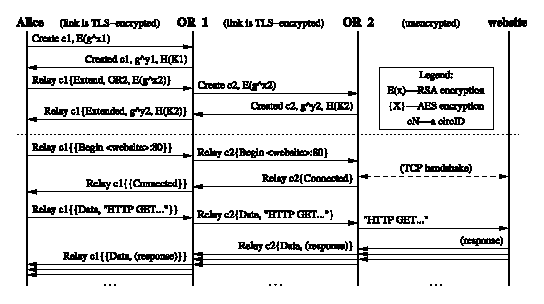
\includegraphics[width=0.9\textwidth]{images/Tor/tap.eps}
	\caption{The Tor Authentication Protocol negotiated over two onion routers. Following circuit construction, Alice sends a HTTP request to the target server, which is encrypted by each router as it travels back up the circuit.\cite{dingledine2004tor}\cite{ling2013protocol}}
\end{figure}

Thus for each router in the circuit, Alice perform one public-key encryption and her half of a Diffie-Hellman-Merkle (DHE) handshake, and each router in turn performs one private-key decryption and their half of a DHE handshake. Under the assumptions that RSA is one way, AES remains unbroken, and $ f $ is strong and acts as a random oracle, an attacker has only a negligible chance of being able to impersonate $ R_{i} $ and read messages that she tunnels through the circuit.\cite{goldberg2006security}

\subsubsection{NTor}

In mid 2013, TAP was superseded by NTor, a new protocol invented by Goldberg, Stebila, and Ustaoglu.\cite{goldberg2013anonymity} Compared to TAP, NTor replaced the computational cost associated with DHE exponentiation with significantly more efficient elliptic curve cryptography (ECC). Its implementation uses Curve25519,\cite{bernstein2006curve25519} a Montgomery curve designed by Bernstein for high-speed ECDHE key exchanges. All Curve25519 operations are implemented to run in $ \mathcal{O}(1) $ time.

NTor is initialized by defining the following,

\begin{itemize}
	\item Let $ H(x,k) $ be HMAC-SHA256, which accepts a message $ x $ and yield a 32-byte MAC output. Let $ k_{1} $, $ k_{2} $, and $ k_{3} $ be some fixed secret keys for the HMAC algorithm, $ k_{1} \neq k_{2} \neq k_{3} $.
	\item Let $ \mathit{C}_{\mathit{gen}}() $ generate a Curve25519 keypair. This function requires 32 bytes from a cryptographically secure source (such as a CSPRNG) to generate the private key, then it derives the public key.
	\item Let $ \mathit{C}_{\mathit{sec}}(pvt, pub) $ yield a 32-byte common secret given a Curve25519 private and public key, $ pvt $ and $ pub $, respectively.
	\item Let each Tor router $ R_{j} $ generate $ b_{j},B_{j} = \mathit{C}_{\mathit{gen}}() $ and publish $ B_{j} $ through the consensus document.
	\item Let $ \mathit{id} $ by the router's identification fingerprint.
\end{itemize}

Then NTor proceeds as:

\begin{enumerate} % 216-ntor-handshake.txt
	\item \label{item:First2}
		\begin{enumerate}
			\item Alice selects a Tor router, $ R_{i} $.
			\item Alice generates $ x,X = C_{\mathit{gen}}() $ and sends $ X $ to $ R_{i} $.
		\end{enumerate}
	\item
		\begin{enumerate}
			\item $ R_{i} $ generates $ y,Y = C_{\mathit{gen}}() $.
			\item $ R_{i} $ sets $ \mathit{sec} = C_{\mathit{sec}}(y, X) \concat C_{\mathit{sec}}(b, X) \concat \mathit{id} \concat X \concat Y $.
			\item $ R_{i} $ computes $ \mathit{seed} = H(\mathit{sec, k_{1}}) $.
			\item $ R_{i} $ computes $ \mathit{auth} = H(H(\mathit{sec, k_{2}}) \concat id \concat B \concat Y \concat X, k_{3}) $.
			\item $ R_{i} $ sends $ Y $ and $ \mathit{auth} $ to Alice.
			\item $ R_{i} $ deletes the $ y,Y $ keypair.
		\end{enumerate}
	\item
		\begin{enumerate}
			\item Alice sets $ \mathit{sec} = C_{\mathit{sec}}(x, Y) \concat C_{\mathit{sec}}(x, B) \concat \mathit{id} \concat X \concat Y $.
			\item Alice computes $ \mathit{seed} = H(\mathit{sec, k_{1}}) $.
			\item Alice confirms that $ \mathit{auth} = H(H(\mathit{sec, k_{2}}) \concat id \concat B \concat Y \concat X, k_{3}) $.
		\end{enumerate}
	\item
		Alice and $ R_{i} $ now have a shared secret $ \mathit{seed} $ that is then used indirectly for symmetric key encryption.	
\end{enumerate}

\subsection{Consensus Documents}
\label{sec:ConsensusDocs}

As previously mentioned, early mixnets and onion routers either assumed a static network topology or flooded updates across the network. By contrast, Tor's network is maintained by a small set of semi-trusted directory authorities. Periodically, Tor routers upload digitally signed ``descriptors'' to these authorities. A descriptor may contain essential routing numbers, router capabilities, cryptographic keys, bandwidth history, or other information.

Each directory authority maintains an long-term authority key (distinct from its normal identity key if it is a Tor router) and a medium-term signing key. Periodically, each directory authority 

\begin{enumerate}
	\item Aggregates the descriptors into a single ``status vote'' document.
	\item Signs its vote with its signing key.
	\item Exchanges its vote and signature with all other authorities.
	\item Computes a single network status consensus from all the other voting documents.
	\item Signs the network consensus and exchanges the signature with all other authorities.
\end{enumerate}

Once this is complete, the consensus is published and is available for download. If clients have knowledge of the Tor network, they may download the more recent consensus from the directory-mirroring routers. By this system, new routers or changes to existing routers can be propagated to all parties within a very short timeframe. Although routers can optionally publish additional non-essential descriptors, clients and routers typically only need the essential descriptors containing routing information, directory signing keys, and router keys. We discuss the documents containing these descriptors below:\cite{TorCollector}\cite{TorDirSpec}

\subsubsection{cached-certs}

The \emph{cached-certs} document contains the long-term authority identity keys and the medium-term signing keys from each directory authority. The Tor source includes the long-term keys, so all parties can verify the authenticity of the signing keys and in turn the descriptors signed by them. They will believe router descriptors if more than half of the authorities have signed it. Each certificate contains the following fields:

\begin{itemize}
	\item \textbf{fingerprint:} The SHA-1 hash of the identity key.
	\item \textbf{dir-key-published:} The time in UTC when the keys were last published.
	\item \textbf{dir-key-expires:} The time in UTC when the signing keys expire.
	\item \textbf{dir-identity-key:} The identity key, typically a 3072-bit RSA key.
	\item \textbf{dir-signing-key:} The signing key, typically a 2048-bit RSA key.
	\item \textbf{dir-key-crosscert:} The signature of the identity key, made using the signing key.
	\item \textbf{dir-key-certification:} The signature of the above fields, made using the identity key.	
\end{itemize}

\subsubsection{cached-microdesc-consensus}

The \emph{cached-microdesc-consensus} document contains network status information. The document includes a header and then a list of condensed descriptors from each router, called microdescriptors. The header includes the following fields:

\begin{itemize}
	\item \textbf{valid-after} (VA), \textbf{fresh-until} (FU), and \textbf{valid-until} (VU). Three timestamps in UTC, $ \mathrm{VA} < \mathrm{FU} < \mathrm{VU} $. VA and VU specifies the earliest and latest time that these descriptors are valid, respectively. All three values are chosen such that two consensuses overlap: $ \mathrm{consensus}_{x} $ will be considered fresh until $ \mathrm{consensus}_{x+1} $ becomes valid, and then $ \mathrm{consensus}_{x} $ expires when $ \mathrm{consensus}_{x+1} $ is no longer fresh.
	\item \textbf{client-versions} and \textbf{server-versions:} An ascending list of recommended Tor versions for clients and routers, respectively.
	\item A list of directory authorities, each containing:
		\begin{itemize}
			\item \textbf{dir-source:} The authority's nickname, fingerprint, IP address, onion routing port, and directory port.
			\item \textbf{contact:} Optional contact information for the authority operator.
			\item \textbf{vote-digest:} The hash of the authority's status vote document.
		\end{itemize}
\end{itemize}

Following the header, each microdescriptor contains:

\begin{itemize}
	\item \textbf{r:} The router's nickname, fingerprint, time of last restart, IP address, onion routing port, and directory port.
	\item \textbf{m:} The SHA-256 hash of the router's microdescriptor. This also includes its entries in the \emph{cached-microdescs} document (discussed below).
	\item \textbf{s:} A list of the router's status flags, as given by the directory authorities. Common examples include Running, Valid, Fast, Guard, Stable, and Exit.
	\item \textbf{v:} The version of the Tor software that the router is running, as reported by the router.
	\item \textbf{w:} The estimated bandwidth that this router is capable of. This value is determined by speed tests from bandwidth authorities, who are a subset of the directory authorities.
\end{itemize}

\subsubsection{cached-microdescs}

The \emph{cached-microdescs} document contains cryptographic keys from each Tor router. Each entry contains:

\begin{itemize}
	\item \textbf{onion-key:} The router's public RSA key, primarily used for TAP authentication.
	\item \textbf{ntor-onion-key:} The router's public Curve25519 key, primarily used for NTor.
	\item \textbf{family:} The fingerprint of routers also under the operator's administration; Tor clients will not construct circuits through any routers that have the same family or that are in the same /16 IPv4 block.
	\item \textbf{id:} The router's fingerprint.
\end{itemize}

\subsection{Hidden Services}
\label{sec:HiddenServices}

Although Tor's primary and most popular use is for secure access to the traditional Internet, Tor also supports \emph{hidden services} -- anonymous servers hosting services such as websites, marketplaces, or chatrooms. These servers intentionally mask their IP addresses through Tor circuits and thus cannot normally be accessed outside the context of Tor. In contrast to Tor-anonymized web requests where the client is anonymous but the server is known, Tor hidden services provide bidirectional anonymity where both parties remain anonymous and never directly communicate with one another.\cite{nicolussi2011human}

Tor does not contain a DNS system for its websites; instead hidden service addresses are algorithmically generated by generating the SHA-1 hash of their public RSA key, truncating to 80 bits, and converting the remainder to base58. Ignoring the possibility of SHA-1 collisions, this builds a one-to-one relationship between a hidden service's public key and its address which can be confirmed without requiring any identifiable information or central authorities. The address is the appended with the .onion Top-Level Domain (TLD).

A hidden server, Bob, first builds Tor circuits to several random relays and enables them to act as \textit{introduction points} by giving them its public key, $ B_{K} $. He then then uploads his public key and the fingerprint identity of these nodes to a distributed hashtable inside the Tor network, signing the result. He then publishes his hidden service address in a backchannel. When Alice obtains this address and enters it into a Tor-enabled browser, her software queries this hashtable, obtains $ B_{K} $ and Bob's introduction points, and builds a Tor circuit to one of them, $ ip_{1} $. Simultaneously, the client also builds a circuit to another relay, $ rp $, which she enables as a rendezvous point by telling it a one-time secret, $ sec $. During this procedure, hidden services must continue to use their same entry node in order to avoid leaking its IP address to possibly malicious onion routers.\cite{bauer2007low}\cite{overlier2006locating}

%\begin{figure}[htdp]
%	\begin{minipage}[b]{0.45\linewidth}
%		\centering
%		\includegraphics[width=\textwidth]{images/Tor/tor-hidden-service-4-higher.png}
%		\caption{Alice uses the encrypted cookie to tell Bob to switch to $ rp $.}
%	\end{minipage}
%	\hspace{0.5cm}
%	\begin{minipage}[b]{0.45\linewidth}
%		\centering
%		\includegraphics[width=\textwidth]{images/Tor/tor-hidden-service-6.png}
%		\caption{Bidirectional communication between Alice and the hidden service.}
%	\end{minipage}
%\end{figure}

She then sends to $ ip_{1} $ a cookie encrypted with $ B_{K} $, containing $ rp $ and $ sec $. Bob decrypts this message, builds a circuit to $ rp $, and tells it $ sec $, enabling Alice and Bob to communicate. Their communication travels through six Tor nodes: three established by Alice and three by Bob, so both parties remain anonymous. From there traditional HTTP, FTP, SSH, or other protocols can be multiplexed over this new channel.

As of March 2015, Tor hosts approximately 25,000 unique hidden services that together generate around 450 Mbit/s of traffic.\cite{TorMetrics}

\section{Motivation}
\label{sec:Motivation}

As Tor's hidden service addresses are algorithmically derived from the service's public RSA key, there is at best limited capacity to select a human-meaningful name. Some hidden service operators have attempted to work around this issue by finding an RSA key by brute-force that generates a partially-desirable hidden service address (e.g. ``example0uyw6wgve.onion'') and although some alternative encoding schemes have been proposed, (section \label{sec:EncodingSchemes}) the problem generally remains. The usability of hidden services is severely challenged by their non-intuitive and unmemorable base58-encoded domain name. For example, 3g2upl4pq6kufc4m.onion is the address for the DuckDuckGo search engine, \\ suw74isz7wqzpmgu.onion is a WikiLeaks mirror, and 33y6fjyhs3phzfjj.onion and \\ vbmwh445kf3fs2v4.onion are both SecureDrop instances for anonymous document submission. These addresses maintain strong privacy as the strong association between its public key and its address significantly breaks the association between the service's purpose and its address. However, this privacy comes at a cost: it is impossible to classify or label a hidden service's purpose in advance, a fact well known within Tor hidden service communities. Over time, third-party directories -- both on the Clear and Dark Internets -- appeared in attempt to counteract this issue, but these directories must be constantly maintained and furthermore this approach is not convenient nor does it scale well. This suggests the strong need for a more complete and reliable solution.

\section{Contributions}

Our contribution to this problem is six-fold:

\begin{itemize}
	\item We introduce a novel distributed naming system that enables Tor hidden service operators to choose a unique human-meaningful domain name and construct a strong association between that domain name and their hidden service address, squaring Zooko's Triangle (section \ref{sec:ZookosTriangle}).
	\item We described a new distributed, publicly confirmable, and partially self-healing transactional database.
	\item We provide OnioNS as a Tor plugin and rely on the existing Tor network and other infrastructure, rather than introduce a new network. This simplifies our assumptions and reduces our threat model to attack vectors already known and well-understood on the Tor network.
	\item We introduce a novel protocol for proving the non-existence of any domain name.
	\item We enable Tor clients to verify the authenticity of a domain name against its corresponding hidden service address with minimal data transfers and without requiring any additional queries.
	\item We preserve the privacy of both the hidden service and the anonymity of Tor clients connecting to it.
\end{itemize}

	
\chapter{\uppercase{Background}}

\section{Tor}

The Tor network is a third-generation onion routing system, originally designed by the U.S. Naval Research Laboratory for protecting sensitive government communication, but today it continues to see global widespread use. Tor refers both to the client-side multiplexing software and to the worldwide volunteer-run network of over six thousand nodes. The Tor software provides an anonymity and privacy layer to end-users by relaying TCP traffic through a series of relays on the Tor network. Tor's encryption and routing protocols are designed to make it very difficult for an adversary to correlate an end user to their traffic. Tor has been recognized by the NSA as the "the king of high secure, low latency Internet anonymity".

\subsection{Design}

Tor routes encrypted TCP/IP user traffic through a worldwide volunteer-run network of over six thousand relays. Typically this route consists of a carefully-constructed three-hop path known as a \textit{circuit}, which changes over time. These nodes in the circuit are commonly referred to as \textit{guard node}, \textit{middle relay}, and the \textit{exit node}, respectively. Only the first node is exposed to the origin of TCP traffic into Tor, and only the exit node can see the destination of traffic out of Tor. The middle router, which passes encrypted traffic between the two, is unaware of either. The client negotiates a separate TLS connection with each node at a time, and traffic through the circuit is decrypted one layer at a time. As such, each node is only aware of the machines it talks to, and only the client knows the identity of all three nodes used in its circuit, making traffic correlation much more difficult difficult compared to a VPN, proxy, or a direct TLS connection.

The Tor network is maintained by nine authority nodes, who each vote on the status of nodes and together hourly publish a digitally signed consensus document containing IPs, ports, public keys, latest status, and capabilities of all nodes in the network. The document is then redistributed by other Tor nodes to clients, enabling access to the network. The document also allows clients to authenticate Tor nodes when constructing circuits, as well as allowing Tor nodes to authenticate one another. Since all parties have prior knowledge of the public keys of the authority nodes, the consensus document cannot be forged or modified without disrupting the digital signature.\cite{Xin2009}

\subsection{Routing}

In traditional Internet connections, the client communicates directly with the server. TLS encryption cannot hide IP and TCP headers, which must be exposed to allow routing. Eeavesdroppers can track end-users by monitoring these headers, easily correlating clients to the their activities. Tor combats this by routing end user traffic through a randomized circuit through the network of relays. The client software first queries an authority node or a known relay for the latest consensus document. Next, the Tor client chooses three unique and geographically diverse nodes to use. It then builds and extends the circuit one node at at time, negotiating respective TLS connections with each node in turn. No single relay knows the complete path, and each relay can only decrypt its layer of decryption. In this way, data is encrypted multiple times and then is decrypted in an onion-like fashion as it passes through the circuit.

\begin{figure}[htdp]
	\begin{minipage}[b]{0.45\linewidth}
		\centering
		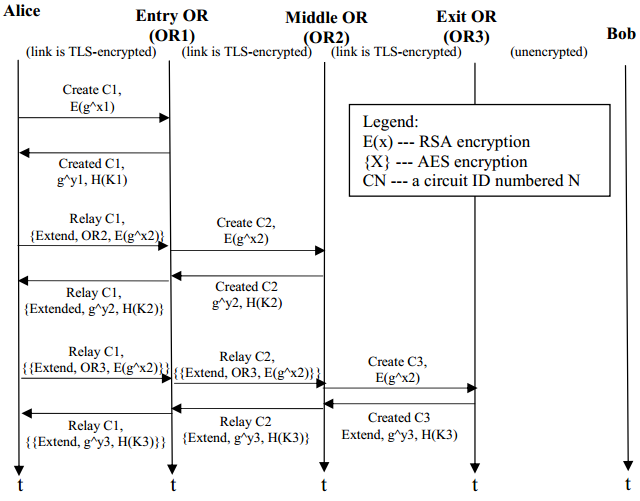
\includegraphics[width=\textwidth]{images/circuit-construction.png}
		\caption{Anatomy of the construction of a Tor circuit.}
		\label{fig:figure1}
	\end{minipage}
	\hspace{0.5cm}
	\begin{minipage}[b]{0.45\linewidth}
		\centering
		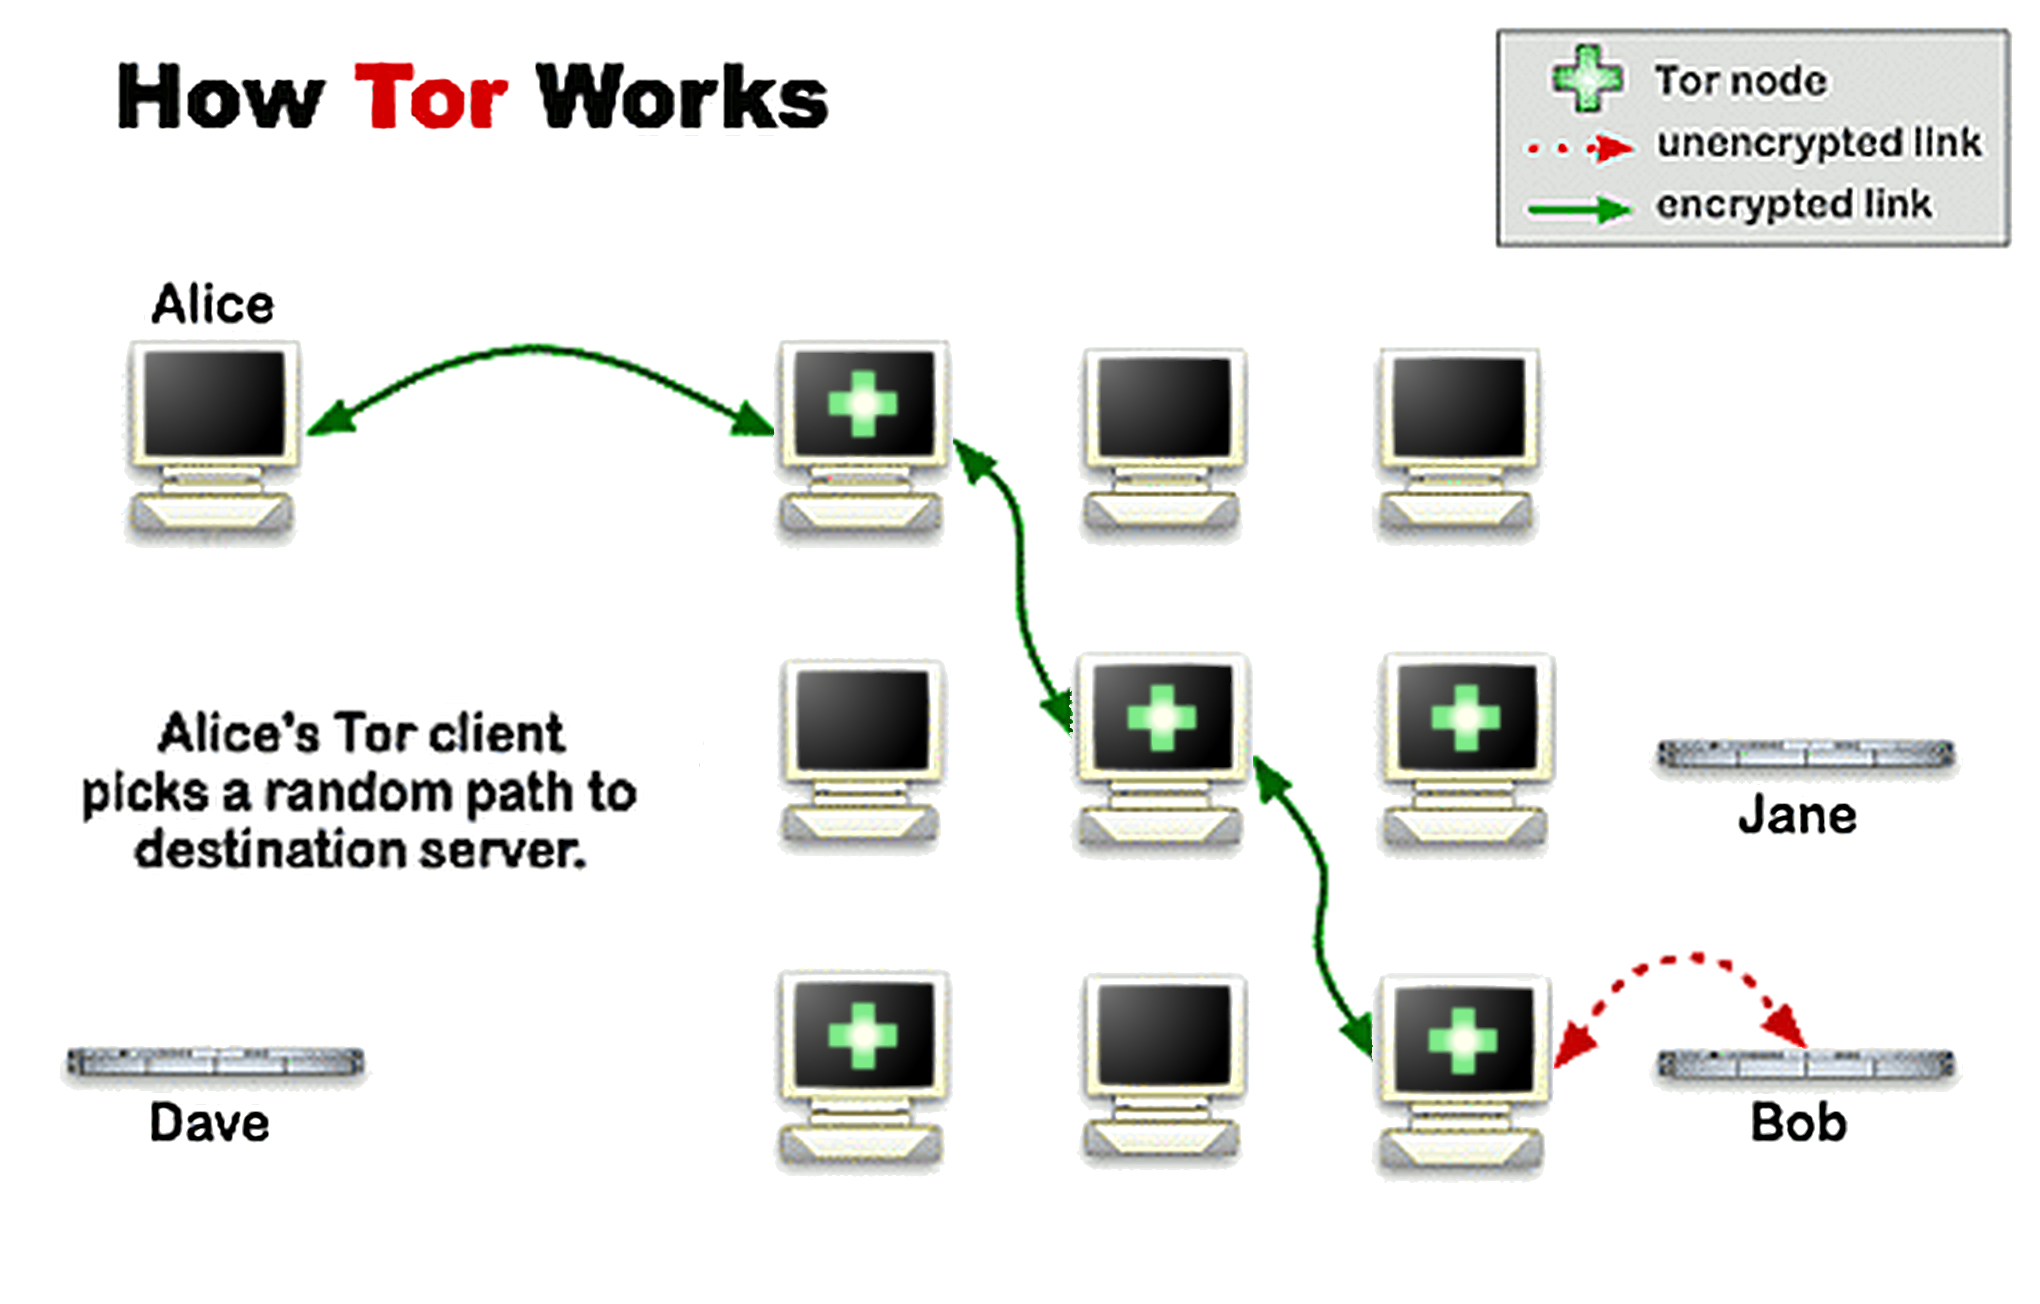
\includegraphics[width=\textwidth]{images/circuit-building-2-5.png}
		\caption{A circuit through the Tor network.}
		\label{fig:figure2}
	\end{minipage}
\end{figure}

The client first establishes a TLS connection with the first relay, $R_{1}$, using the relay's public key. The client then performs an ECDHE key exchange to negotiate $K_{1}$ which is then used to generate two symmetric session keys: a forward key $K_{1,F}$ and a backwards key $K_{1,B}$. $K_{1,F}$ is used to encrypt all communication from the client to $R_{1}$ and $K_{1,B}$ is used for all replies from $R_{1}$ to the client. These keys are used conjunction with the symmetric cipher suite negotiated during the TLS handshake, thus forming an encrypted tunnel with perfect forward secrecy. Once this one-hop circuit has been created, the client then sends $R_{1}$ the RELAY\_EXTEND command, the address of $R_{2}$, and the client's half of the Diffie-Hellman-Merkle protocol using $K_{1,F}$. $R_{1}$ performs a TLS handshake with R${2}$ and uses $R_{2}$'s public key to send this half of the handshake to $R_{2}$, who replies with his second half of the handshake and a hash of $K_{2}$. $R_{1}$ then forwards this to the client under $R_{1,B}$ with the RELAY\_EXTENDED command to notify the client. The client generates $K_{1,F}$ and $K_{1,B}$ from $K_{2}$, and repeats the process for $R_{3}$,\cite{Ling2012} as shown in Figure 3. The TCP/IP connections remain open, so the returned information travels back up the circuit to the end user.

Following the complete establishment of a circuit, the Tor client software then offers a Secure Sockets (SOCKS) interface on localhost which multiplexes any TCP traffic through Tor. At the application layer, this data is packed and padded into equally-sized Tor \textit{cells}, transmission units of 512 bytes. As each relay sees no more than one hop in the circuit, in theory neither an eavesdropper nor a compromised relay can link the connection's source, destination, and content. Tor further obfuscates user traffic by changing the circuit path every ten minutes,\cite{McCoy2008} as shown in Figure 4. A new circuit can also be requested manually by the user.

\begin{figure}[htbp]
	\centering
	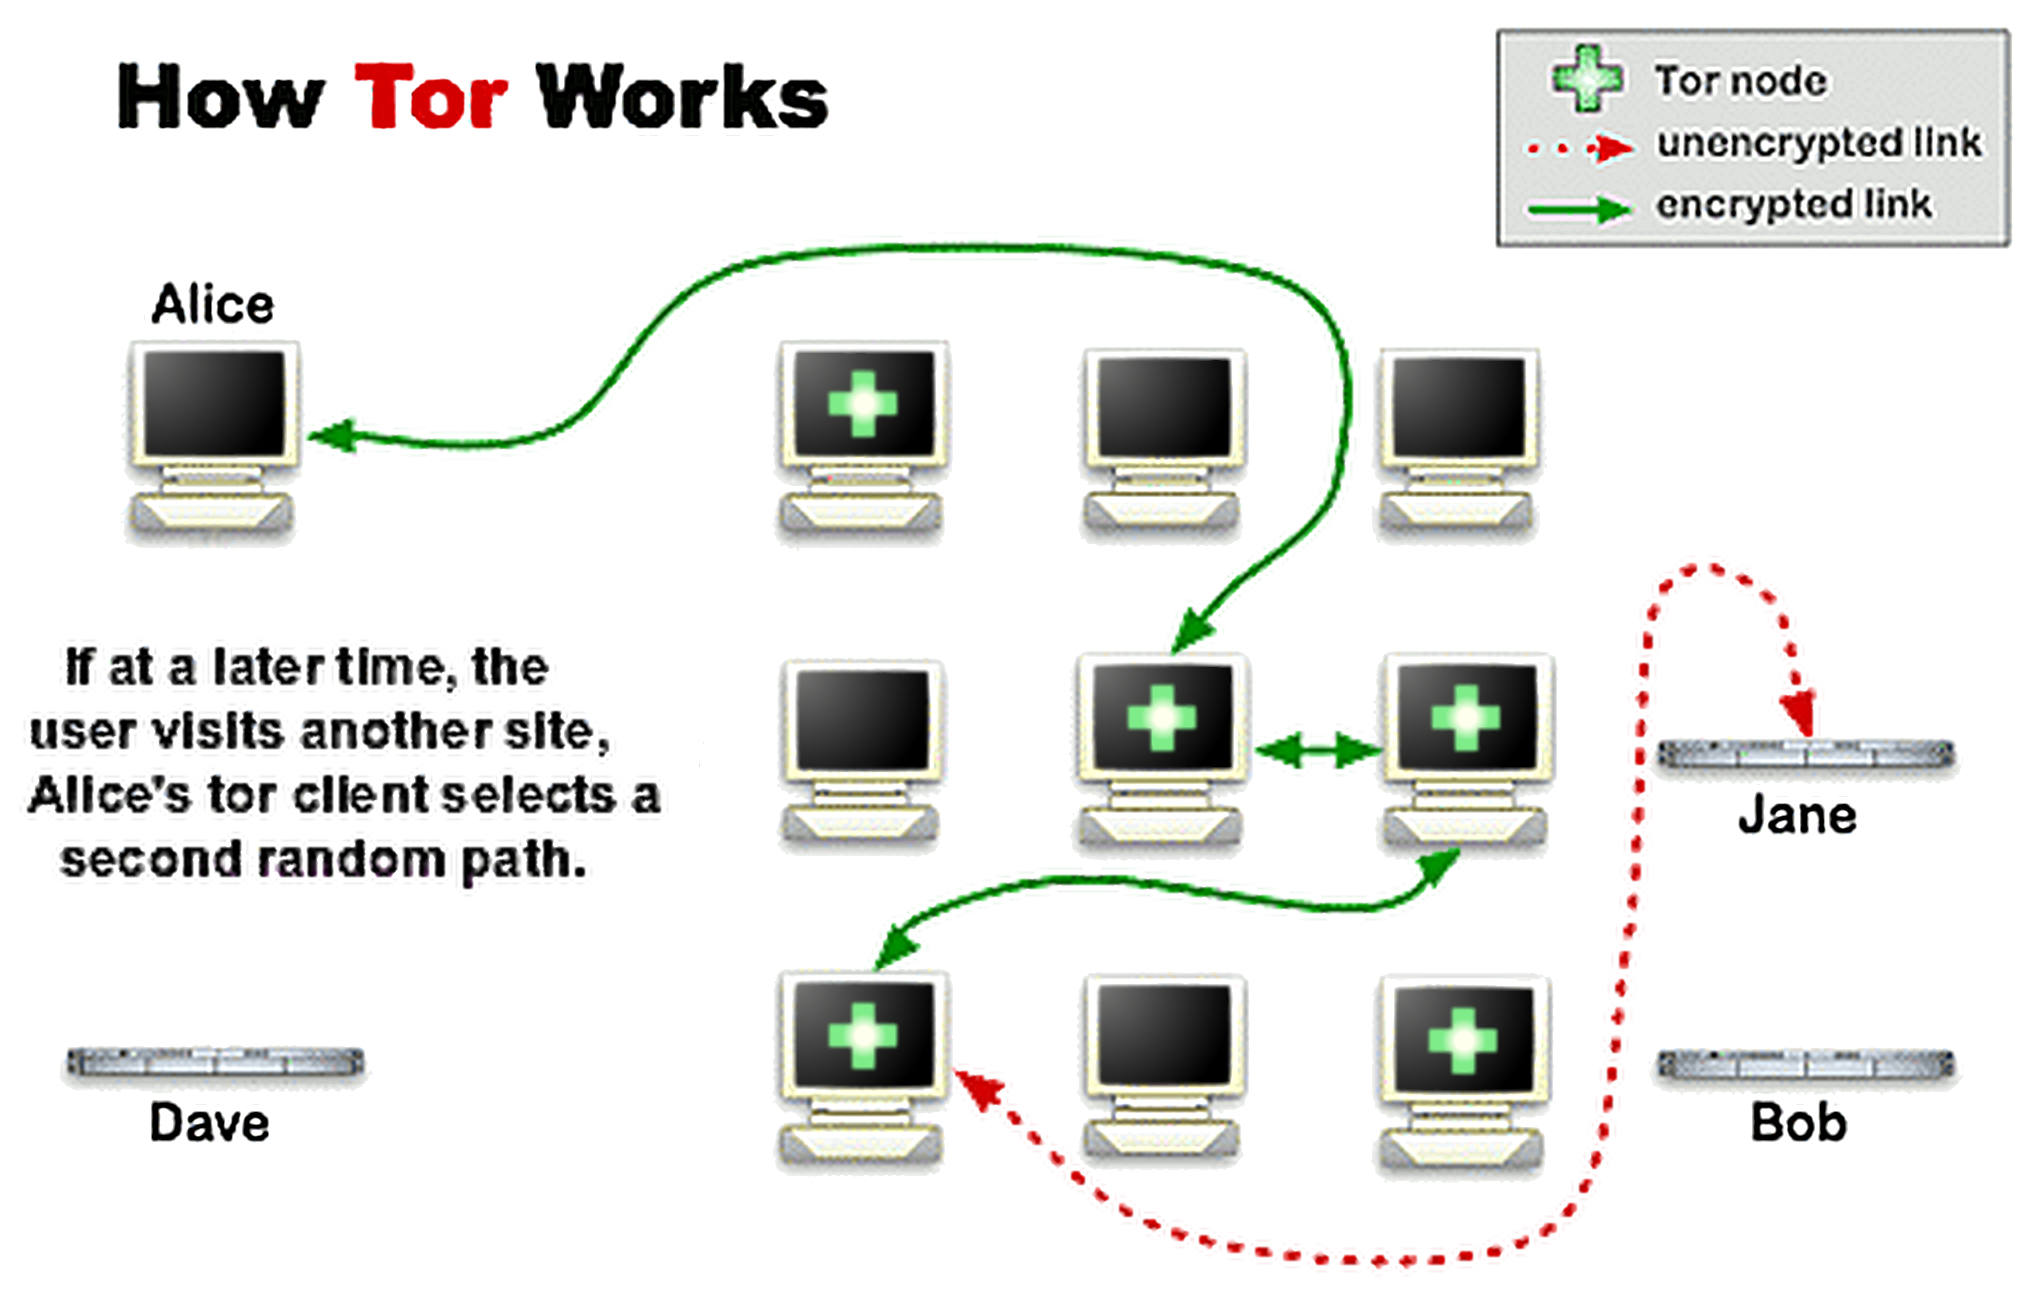
\includegraphics[width=0.6\textwidth]{images/circuit-change-1-4.png}
	\caption{A Tor circuit is changed periodically, creating a new user identity.}
	\label{fig:figure3}
\end{figure}

% Although a different guard node is used here, in practice the choice of entry point is preserved for extended periods of time.

Tor users typically use the Tor Browser, a custom build of Mozilla Firefox with a focus on security and privacy. The TBB anonymizes and provides privacy to the user in many ways. These include blocking all web scripts not explicitly whitelisted, forcing all traffic including DNS requests through the Tor SOCKS port, mimicking Firefox in Windows both with a user agent (regardless of the native platform) and SSL cipher suites, and reducing Javascript timer precision to avoid identification through clock skew. Furthermore, the TBB includes the Electronic Frontier Foundation's HTTPS Everywhere extension, which uses regular expressions to rewrite HTTP web requests into HTTPS for domains that are known to support HTTPS. If this is the case, an HTTPS connection will be established with the web server. If this happens, end-to-end encryption is complete and an outsider near the user would be faced with up to four layers of TLS encryption: $K_{1,F}(K_{2,F}(K_{3,F}(K_{server}(\textrm{client\ request}))))$ and likewise $K_{1,B}(K_{2,B}(K_{3,B}(K_{server}(\textrm{server\ reply}))))$ for the returning traffic, making traffic analysis very difficult.

\subsection{Hidden Services}

Although Tor's primary and most popular use is for secure access to the traditional Internet, Tor also supports anonymous services, such as websites, marketplaces, or chatrooms. These are a part of the Dark Web and cannot be normally accessed outside the context of Tor. In contrast to Tor-anonymized web requests where the client is anonymous but the server is known, Tor hidden services provide bidirectional anonymity where both parties remain anonymous and never directly communicate with one another. This allows for a greater range of communication capabilities. Tor's hidden service protocol was introduced in 2004 and has not seen a major revision since then.\cite{NicolussiThesis2011}

Tor hidden services are known only by their public RSA key. Tor does not contain a DNS system for its websites; instead the domain names of hidden services are an 80-bit truncated SHA-1 hash of its public key, postpended by the .onion Top-Level Domain. Once the hidden service is contacted and its public key obtained, this key can be checked against the requested domain to verify the authenticity of the service server. This process is analogous to SSL certificates in the clearnet, however Tor's authenticity check leaks no identifiable information about the anonymous server. If a client obtains the hash domain name of the hidden service through a backchannel and enters it into the Tor Browser, the hidden service lookup begins.

Preceding any client communication, the hidden server, Bob, first builds Tor circuits to several random relays and enables them to act as \textit{introduction points} by giving them its public key, $B_{K}$. The server then uploads its public key and the fingerprint identity of these nodes to a distributed hashtable inside the Tor network, signing the result. When a client, Alice, requests contact with Bob, Alice's Tor software queries this hashtable, obtains $B_{K}$ and Bob's introduction points, and builds a Tor circuit to one of them, $IP_{1}$. Simultaneously, the client also builds a circuit to another relay, $RP$, which she enables as a rendezvous point by telling it a one-time secret, $S$.

\begin{figure}[htdp]
	\begin{minipage}[b]{0.45\linewidth}
		\centering
		\includegraphics[width=\textwidth]{images/tor-hidden-service-4-higher.png}
		\caption{Alice uses the encrypted cookie to tell Bob to switch to $RP$.}
		\label{fig:figure4}
	\end{minipage}
	\hspace{0.5cm}
	\begin{minipage}[b]{0.45\linewidth}
		\centering
		\includegraphics[width=\textwidth]{images/tor-hidden-service-6.png}
		\caption{Bidirectional communication between Alice and the hidden service.}
		\label{fig:figure5}
	\end{minipage}
\end{figure}

She then sends to $IP_{1}$ an cookie encrypted with $B_{K}$, containing $RP$ and $S$. Bob decrypts this message, builds a circuit to $RP$, and tells it $S_{1}$, enabling Alice and Bob to communicate. Their communication travels through six Tor nodes: three established by Alice and three by Bob, so both parties remain anonymous. From there traditional HTTP, FTP, SSH, or other protocols can begin, multiplexed over this new channel.

\section{Motivation}

The usability of hidden services is severely challenged by their non-intuitive 16-character hexadecimal domain names: 3g2upl4pq6kufc4m.onion is the address for the DuckDuckGo hidden service, whereas 33y6fjyhs3phzfjj.onion is the Guardian's SecureDrop service for anonymous document submission, and blockchainbdgpzk.onion is the anonymized edition of blockchain.info. It is rarely clear what service a hidden server is providing by its domain name alone without relying on third-party directories for the correlation, directories which must be updated and reliably maintained constantly. These must be then distributed through backchannels such as /r/onions, the-hidden-wiki.com, or through a hidden service that is known in advance.

One attempt at alleviating the issue is to generate hidden service many RSA keys in an attempt to find one whose hash contains or begins with a meaningful name. This is the case with Blockchain.info's hidden service, although such attempts are time-consuming and only partially effective because the size of the domain keyspace is too large to be effectively brute-forced in any reasonable length of time. Tor Proposal 224 makes this solution even worse as it suggests 32-byte domain names which embed the entire hidden service key in base32. Although prefixing the domain name with a meaningful word helps identify a hidden service, it does nothing to alleviate the logistic problems of entering a hidden service domain name manually into the Tor Browser, an issue that is not shared by domains in the clearnet.

It is clear that the usability problem exists and none of the few attempts to solve it have been fully successful. It is for these reasons that I propose EsgalDNS as a full solution.

	% Be sure to write chapter titles in ALL CAPS
\chapter{\uppercase{DISCUSSION}}
\thispagestyle{empty}

\section{Objectives}

A high degree of anonymity, privacy, and security are of paramount importance for all Tor users. This context makes the inclusion of additional capabilities challenging. To meet these challenges and to remain acceptably resistant to attack, any proposed DNS system for Tor hidden services must meet at least the following requirements: %Tor is a high-anonymity, high-privacy, censorship-resistance tool. 

\begin{enumerate}
	\item The registrations must be anonymous. It should be infeasible to identify the registrant from the registration, including over the wire.
	\item Lookups must be anonymous. Clients must stay anonymous when looking up registrations, otherwise they leak what hidden services they are after.
	\item Registrations must be publicly confirmable. Akin to SSL certificates on the clearnet, clients must be able to verify that the registration matches and came from the service they are after, and is not a forgery.
	\item It must be distributed. The Tor community will adamantly reject any centralized solution for Tor hidden services, as they have in the past for other proposals.
	\item It must remain simple to use. Most Tor users are not security experts and Tor puts almost all cryptographic details and routing details behind the scenes.
	\item It must remain backwards compatible. The existing Tor hidden service infrastructure must still remain functional.
	\item It should not be possible to maliciously modify or falsify registrations in the database or in transit, even though insider attacks.
\end{enumerate}

There are a couple of works in the literature regarding a DNS system for Tor, none of which fully solve all of these problems.

\section{Solutions Analysis}

1. Hidden services sign registration, upload using Tor to blockchain. Upload IP node so it can be contacted directly. Fully completes triangle.
2. 1 except clients using Tor download blockchain, find info they are after.
3. 2 except clients query Tor nodes for block, use it.
4. 3 except clients contain hashes/nonces that can be used to verify each block. Nodes also return onion as well to improve efficiency ahead of block download.

\section{Conclusion}

4 is best overall, 1 still possible as option.
	% Be sure to write chapter titles in ALL CAPS
\chapter{\uppercase{PROPOSAL}}
\thispagestyle{empty}

My proposal...

	
\chapter{IMPLEMENTATION}

\section{Prototype Design}

We have developed a prototype of OnioNS and have implemented most of the hidden service, server, and client protocols in C++11. We package the software on the Launchpad online build system and support Linux Debian and derivates such as Ubuntu and Linux Mint. We use the Botan library for cryptographic operations, with the Mersenne Twister provided through the C++ Standard Template Library (STL). We have made our software online at github.com/Jesse-V/OnioNS. Our reference implementation uses the libjsoncpp header-only library for encoding and decoding purposes. The library is also available as the libjsoncpp-dev package in the Debian, Ubuntu, and Linux Mint repositories.

\section{Experimentation}


\emph{Todo: I will carry out experiments in test deployments of the Tor network and see what the demand is. I anticipate it being relatively lightweight. The proof-of-work will almost certainly be the computational bottleneck.}

\emph{Bandwidth, CPU, RAM, latency for clients to be determined...}

%demand on participating nodes to be determined...

%Unlike Namecoin, OnionNS' \emph{page}-chain is of $ L $ days in maximal length. This serves two purposes:

%\begin{enumerate}
%	\item Causes domain names to expire, which reduced the threat of name squatting.
%	\item Prevents the data structure from growing to an unmanageable size.
%\end{enumerate}

\subsection{Proof-of-work}

\emph{What are the optimal parameters for scrypt? What are the implications of setting it too high or too low?}

\emph{How much bandwidth and time does this take?}

\emph{How does the bandwidth and CPU load scale in response to a larger Quorum? Assuming reasonable clockskew, how off will the exchanges be? Are there any race conditions that need to be resolved?}

\emph{Queres: How long does this take, and how can we improve efficiency? Can clients on even low-end hardware calculate the proof-of-work?}


\section{Results}


\emph{This will be expanded/rewritten once I finish implementation and deploy it in test/prototyping networks. I plan on using Chutney.}

	% Be sure to write chapter titles in ALL CAPS
\chapter{\uppercase{EXPERIMENTS}}

\section{Research Questions}
There are four main questions of focus that the following experiments attempt to answer:
\begin{enumerate}
	\item What is the impact on the size of the test suite using abstract URLs instead of an exhaustive enumeration of every variable combination?
	\item What is the fault finding effectiveness of testing with abstract URLs versus exhaustive testing?
	\item What is the impact on the size of the test suite using combinatorial coverage compared to single coverage?
	\item What is the fault finding effectiveness of the combinatorial coverage compared with single coverage?
\end{enumerate}

\section{Sample Application}
All experiments were conducted on a sample Rich Web Application written by the author and is available at \url{http://chadmaughan.com/thesis}.  The application provides United States census information for 1990, 2000, and preliminary numbers from 2005 for each state, county, and city with a population over 25,000 residents.  The application is designed for mobile devices with larger touch points.  The sample application uses the following technologies:

\begin{enumerate}
\item Backbone.js: A client-side, JavaScript MVC framework that gives structure to rich web applications.  Backbone.js allows you to bind custom events to models, and route URL fragments to JavaScript functions.
\item jQuery Mobile: A unified, HTML5-based cross-platform user interface system for mobile devices.  It focuses on semantic markup that is easily themeable.
\item Spring MVC: A module of the popular Spring Framework for Java that allows for easy implementation of server-side controllers for building REST APIs.
\item Apache Derby DB: An open source, embedded relational database implemented in Java.
\end{enumerate}

Source code for both the application and the fault finding, testing code is also available at \url{http://code.chadmaughan.com/thesis}.  Metrics about the sample application are included in Table~\ref{table:sampleAppInfo}.  A sample screenshot of the application is provided in Figure~\ref{fig:screenshot}.

\begin{table}[h]
	\centering
	\caption{Sample Rich Web Application Information.}
	\begin{tabular}{| l | r|}
		\hline
Number of Application States		& 199,484 	\\ \hline
Number of Files				& 328 		\\ \hline
JavaScript Lines of Code			& 605 		\\ \hline
Java Number of Classes			& 21 		\\ \hline
Java Lines of Code				& 1,091 		\\ \hline
Seeded Faults					& 73 		\\ \hline
	\end{tabular}
\label{table:sampleAppInfo}
\end{table}

\begin{figure}[htbp]
\centering
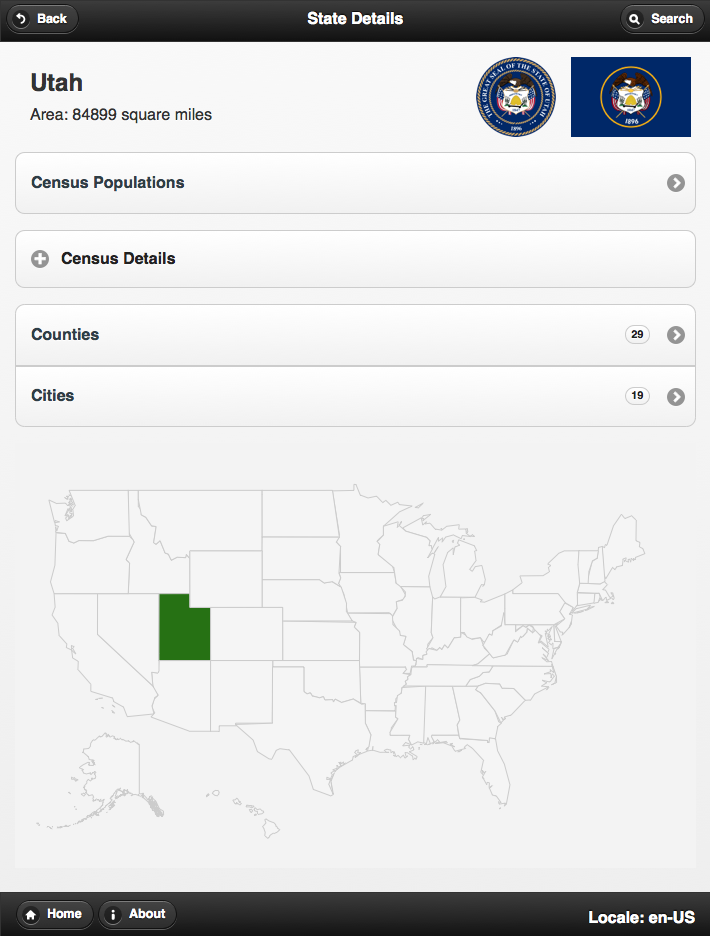
\includegraphics[width=0.9\textwidth]{images/ipad-screenshot.png}
\caption{Sample rich web application screenshot.}
\label{fig:screenshot}
\end{figure}

\section{JavaScript Faults}
The sample application is seeded with 73 faults.  A detailed list of those exceptions and the categories they belong to are listed in Table~\ref{table:seededExceptions}.  

On fault categories, Sampath et al. described five web application fault categories\cite{sampath2007applying}, of which all are used in the sample application.

\begin{enumerate}
\item Data store faults: Faults in the application code that manipulates data in any kind of data store.  This category of faults also applies to data that is incorrectly persisted in the data store.  There are a number of seeded data store faults in the sample application.

\item Logic faults: Faults in the application code that implements business logic and control flow.  An example of this is an error in the page transition with jQuery Mobile. 

\item Form faults: Faults in the application code that controls, modifies and displays name-value pairs in forms.  The sample application does not submit any data to the server but does use dynamically updated forms to direct to different application states.

\item Appearance Faults: faults in the application code that controls the way in which a web page is displayed.  With the use of modern JavaScript based templating solutions, such as Mustache.js and Underscore.js, appearance faults typically cause a template to not be rendered.  The sample application demonstrates this type of error when trying to load the search page.

\item Link faults: Faults in the application code that changes the page pointed to by an URL.
\end{enumerate}

Guo and Sampath \cite{guo2008web} add a sixth category, compatibility faults or ``faults in application code that ensures that the web application complies with different browsers, versions of browsers and other client environments.''  With the rapid introduction of new HTML5 APIs (i.e., Websockets and Webstorage) and the varying speed of adoption among browser creators, compatibility faults will play an increasingly important role in client-side testing.  

Guo also expands the logic faults category to include seven sub-categories.  The sub-categories of logic faults are:

\begin{enumerate}
\item Browser interaction faults: Faults in the application code that control the web browser, such as code that disables the ``back'' button on the browser, or code that is affected by user-defined browser settings, such as disabled cookies.  Browser manipulation is discouraged as it alters expected application behavior.  Other browser settings, such as disabling JavaScript, would render the application useless.  As such, the sample application does not use this fault sub-category.

\item Session faults: Faults in the application code that deal with maintaining state of application or other session-based operations such as using sessions to save and data entered into a form and display the data after the sessions has been validated.  As most rich web applications are stateless to avoid the overhead of session management and allow for greater scalability, the sample application does not use this sub-category.

\item Paging faults: Faults in the application code that deals with paging when displaying large amounts of data on the screen.  While applicable to rich web applications, the sample application does not use this sub-category.

\item Server-side parsing faults: Faults in the application code that deal with server-side parsing of HTML, XML, and JavaScript tags.  This sub-category does not apply to rich web applications as HTML used in a RWA is typically a minimal page used only as an entry point.  ``client-side parsing faults''  are more applicable to rich web applications.   The sample application has a number JavaScript syntax related faults.  These errors are described below in Table~\ref{table:seededExceptions}.

\item Encoding/decoding faults: Faults in the application code that encodes or decodes characters for transmission, storage, and display

\item Locale faults: Faults that exist in application code that sets or gets locale-specific information, such as date format or language.  Not used in the sample application.

\item Other: Other logic faults that do not belong to any of the above sub categories.
\end{enumerate}

More recently, in addition to Sampath and Guo, Ocariza et al. \cite{ocariza2011javascript} defines five categories specifically for JavaScript exceptions.  He found that JavaScript exceptions tend to be much more defined than other applications and fall into well-defined categories.  In fact, 94\% of all errors studied from the Alexa top 100 list fall into five categories, namely:

\begin{enumerate}
\item Permission Denied:  Faults in the application code that attempt to access JavaScript components from another domain violating the same-origin policy.  The sample application has a seeded fault where it tries to load recent search data from Twitter and violates the same-origin policy. 

\item Null Exception faults: Faults in the application code where a property or method is accessed via a null object.  The sample application attempts to add a CSS class name to an element that is null.

\item Undefined Symbol faults: Faults in the application code where a function or variable is accessed that has not been previously defined.

\item Syntax Error faults: Faults in the application code where interpreted code, such as in an eval() function, has the wrong syntax.

\item Miscellaneous faults: Faults in the application code that apply specifically to a single site.
\end{enumerate}

These five categories align more closely with the JavaScript Error object and its six other core errors: EvalError (Syntax Error faults), RangeError, ReferenceError (Undefined Symbol faults), SyntaxError (Syntax Error faults), TypeError, and URIError\cite{mdnError}.

\begin{table}[h]
	\centering
	\caption{Sample Rich Web Application Seeded Errors.}
	\begin{tabular}{| l | p{5cm} | p{3cm} | l |}
		\hline

Location    &    Description    &    Category    &    Count		\\ \hline

index.html:39 	&
console.log(variable) - variable is not defined.  & 
ReferenceError, Undefined& 
1 
\\ \hline

main.js:54	& 
SearchPageView template is not included as a source.  & 
ReferenceError, Appearance&
1 
\\ \hline

geochart:438& 
County Map doesn't exist on County Details page. "Container is not defined" error.  & 
Appearance& 
1 (3,144)
\\ \hline

main.js:49&
Syntax Error on eval() - eval("window.print(;") & 
SyntaxError & 
1 
\\ \hline

main.js:37& 
Missing script file - notthere.js"  & 
Link, Other, Misc& 
1 
\\ \hline

jquery-1.7.1.min.js:4 & 
Multiple words in the name (9 states plus Washington DC) doesn't have a flag to display & 
& 
10 
\\ \hline

jquery-1.7.1.min.js:4 & 
Multiple words in the name (9 states plus Washington DC) doesn't have a seal to display & 
Appearance& 
10 
\\ \hline

CityController.java:39&
Cities with periods in their name/code, return HTTP 500 (i.e., St. George, UT). & 
Data Store & 
13 
\\ \hline

index.html:87& 
Type Error 'bad type' for all Washington State cities & 
TypeError, Misc& 
37 
\\ \hline

twitter.js:4& 
City Twitter Search feed & 
Permission & 
1 (1,267)
\\ \hline

census-table-view.js:17& 
Adds a CSS class to a null element& 
Null Exception, TypeError & 
1
\\ \hline

	\end{tabular}
\label{table:seededExceptions}
\end{table}

\section{Testing Technologies}
In addition to the sample Rich Web Application, the code used to identify the seeded faults rely on some key technologies.  These technologies are listed below:

\begin{enumerate}
\item Neo4j: A powerful graph database with a rich API that was used to both systematically identify variables in semantic URLs and store a full navigation graph of the rich web application for test traversal retrieval.

\item BrowserMob: An embedded proxy software that allows the interception of HTTP requests from the client and HTTP responses from the server.  This allows for the identification of network errors and for the modification of the server responses to assist in identifying client side JavaScript errors.

\item Selenium WebDriver: Allows for the crawling and interaction with the application in the various browsers ``as the user would,'' giving a more accurate result while testing.
\end{enumerate}

\section{Navigation Graph}
A navigation graph is a visual representation of an application\cite{herman2000graph}.  A navigation graph of a rich web application is a visual representation of how different states of the web application are related to one another.  A traditional web application navigation graph typically would have a single node for each HTML page or a single node for each rendering of a server-side script.  An edge on a traditional web application represents an HTML anchor tag.  As rich web applications typically have a single or very limited number of HTML pages acting as entry points, a node in the navigation graph of a rich web application represents a single state of the application.  An edge in a navigation graph for a rich web application represents a transition from one state to another.  Like in a traditional web application, this is also typically done through an HTML anchor tag.

Building a navigation graph of the rich web applications has many benefits, including understanding the application as a whole, maintenance over the development cycle, and test case generation and the subsequent testing of those tests\cite{wang09}.  To build the graph, and expand it as the application increases in size, a rich web application can be crawled using the Selenium WebDriver in a simple depth first traversal.  Figure~\ref{crawlingAlgorithm} demonstrates the crawling algorithm using Selenium WebDriver.

\begin{figure}
\begin{lstlisting}
	public static void main(String[] args) {
		driver = new FirefoxDriver();
		new Crawl("http://example.com");
	}

	public Crawl(String startingUrl) throws Exception {
		String newAddress = null;
		while ((newAddress = queue.poll()) != null)
			processPage(newAddress);
	}

	private void processPage(String sourceHref) throws Exception {
		driver.get(sourceHref);
		List<WebElement> links = driver.findElements(By.tagName("a"));
		Node sourceNode = retrieveOrCreateNode(sourceHref);
		String targetHref;

		for (int i = 0; i < links.size(); i++) {
			WebElement w = links.get(i);		
			targetHref = w.getAttribute("href");
			if (isValidUrl(targetHref)) {
				if(w.isDisplayed()) {
					Node targetNode = retrieveOrCreateNode(targetHref);				
					if(targetNode == null)
						targetNode = nodeMapper.mapNode(targetHref, w);				
					sourceNode.createRelationshipTo(targetNode, 
							RelationshipTypes.LINKS_TO);
					if (!processed.contains(targetHref))
						queue.add(targetHref);
				}
			}
		}
	}
\end{lstlisting}
\caption{Depth first crawling of a rich web application}
\label{crawlingAlgorithm}
\end{figure}

Also of benefit is the ability to identify key, holistic characteristics about the application as the navigation graph is built.  For example, while this experiment does not focus on test prioritization, systematically creating a navigation graph with Selenium WebDriver allows you to easily record and track key information about state transitions in the application.  As an example, one may wish to prioritize testing based on the location of links or elements that trigger a change in state.  Combining the exact top and left pixel location of that element allows you to prioritize links that are more in the key navigation sections.  As another prioritization strategy with a navigation graph, one could also easily prioritize based on states of the application that are most transitioned.

\section{Abstract URLs}
One problem with the depth-first traversal of a rich web application is the time it takes to complete a full application crawl.  For example, the sample census application discussed previously contains nearly 200,000 different states.  Assuming an average page load of around 500 milliseconds, it would still require more than 27 hours to perform a full regression test.  While this amount of time to perform an exhaustive regression test is possible, it may not always be practical.

Using variables previously identified through the algorithm described in the background chapter, application states can be stored in the navigation graph as ``abstract URLs''\cite{wang09}, or URLs with variable names instead of each possible value.  Similar to semantic URL formats discussed earlier, an example of an abstract semantic URL stored in a navigation graph would look as follows:

\begin{figure}[H]
\centering
http://example.com/\#/state/\{var1\}/county/\{var2\}/city/\{var3\}
\end{figure}

Storing the abstract URL instead of every URL variable combination significantly reduces the number of tests required.  Indeed, it is ideal as most rich web application states reuse small HTML templates for the displaying of particular data points.  This means that client-side errors would typically manifest themselves for every variance of a variable.  One disadvantage of using abstract URLs is that data specific errors may be missed.  For example, the sample application has a fault where any city with a period in it's name (i.e., ``St. George, UT'') doesn't render correctly.  Unless the random value for the abstract URL variable selected contained a period, this data related fault would be missed.  While not discussed in detail in this paper, due to the available resource of the full application structure (from the systemic variable identification), one possibility is to use a sample size confidence level to adequately test a certain size of the data available.

One of the experiments completed was calculating and comparing the amount of time required to crawl a full rich web application, a reduced number of states based on a sample size, and a fully reduced test suite testing only abstract URLs one time.  Results of this experiment are discussed in the following chapter.

\section{Capturing Errors}
Another difficulty encountered with testing rich web applications is the ability to identify errors that occur in the browser.  JavaScript errors are difficult to systematically intercept and report.  This section introduces a novel approach for identifying two different types of exceptions during testing, namely network related and JavaScript browser related.

Some network related exceptions are errors that are simple to identify on the server-side by examining the log files.  BrowserMob was used as an embedded proxy to intercept all communications between the browser and the server.  This allows for the logging of network related exceptions, as well as response interception and subsequent modification for JavaScript exception reporting.

JavaScript exceptions in modern browsers typically manifest themselves via the browser console object.  The console is typically not visible to the end user and needs to be enabled via menu options or browser plug-ins such as Firebug for Firefox.  A sample of thrown exception is shown in Figure~\ref{fig:consoleError}.

\begin{figure}[H]

\includegraphics[width=0.9\textwidth]{images/console-error.png}
\caption{An example JavaScript error in the Firebug console.}
\label{fig:consoleError}
\end{figure}

Unfortunately, once these exceptions are thrown, there is no way to retrieve them from the browser.  A simple way to capture these is to introduce a small snippet of JavaScript code in every HTML entry point that has a collection for inserting exceptions.  This requires that testing code be added to the deployable deliverable, considered by many to be bad practice.  As an alternative, this experiment introduces a novel approach to keep testing scaffolding out of the deployable code base.  BrowserMob is used in to intercept only full HTML page responses from the server to the browser, and alter it injecting a custom browser Console object at the beginning of the HTML \textless script\textgreater\  tag.  This custom Console object stores any exception for later retrieval and reporting.  Figure~\ref{consoleJavascript} shows the custom JavaScript injected into each response.

\begin{figure}
\begin{lstlisting}[language=HTML]
	<script type="text/javascript">
		window.jsErrors = [];
		window.onerror = function(errorMessage) {
			window.jsErrors[window.jsErrors.length] = errorMessage;
		}
	</script>
\end{lstlisting}
\caption{Browser exception catching}
\label{consoleJavascript}
\end{figure}

\section{Combinatorial Testing}
The preparation done with the creation of both the exhaustive and the reduced navigation graph has prepared for the generation of combinatorial test cases.  The sample application has some variables, namely state, county, and city, that are hierarchical in nature.  Czerwonka\cite{czerwonka2008pairwise}, while describing the capabilities of the Microsoft PICT combinatorial test generation tool, explains that these hierarchical variables are treated as a ``sub-model'' and pairwise combined first to represent a single variable that is then used in the generation of the combinatorial test cases.  For example, in the sample application on the home page, the State of Utah, Cache County, and Logan City are combined together to form a single variable that is then used in building the combinatorial tests.  Additionally, a great majority of exceptions that occur in rich web applications result from the different browsers and environments.  Tatsumi\cite{grochtmann1995test} made the distinction of input and environment variables.  The input variables discovered via the process introduced previously can then be combined with provided environment variables to also identify ``compatibility faults.''  I discuss in the concluding chapter future work that can add distributed computing capabilities enabling browsers in different client environments to perform the same tests.
	% Be sure to write chapter titles in ALL CAPS
\chapter{\uppercase{RESULTS}}

Results of analysis and of experiments of implementation...
	% Be sure to write chapter titles in ALL CAPS
\chapter{\uppercase{Conclusions}}

Combinatorial testing is a powerful tool in identifying software faults.  Indeed, Kuhn, et al. showed in a study of a NASA Distributed Database that 93\% of all faults were identified by 2-way combinations, and 98\% by 3-way combinations.  Across industries, ``the detection rate curves for the other applications studied are similar, reaching 100\% detection with 4 to 6-way interactions'' \cite{kuhn2010practical}.  

Rich web applications continue to grow with the introduction and rapid development of new HTML5 features and APIs, powerful JavaScript based frameworks, and increasingly more powerful client machines.  This thesis demonstrates that combinatorial testing can play an important role in the testing of rich web applications and that more future work is needed.

While there is not a specific standard for semantic URLs compared to the traditional URL format defined in RFC 1378, this paper has shown a novel way to identify variables by employing graph theory and branching complexity analysis.  This approach worked with the sample application but needs additional work to be universally applicable to all semantic URL formats.  For instance, an application that has a small number of variables that equal the branching complexity of the URL structure could result in false positives with variable identification.

This research also showed that using abstract URLs to generate test cases was an effective and inexpensive way to discover all types of faults except data faults in the sample application and particularly well suited for template heavy client-side applications.  While it didn't find as many errors as the exhaustive or combinatorial approaches, with only 27 tests (0.0001\% of the exhaustive tests run) it found 19.5\%.  Using abstract URLs may be a good strategy when time is extremely limited.  A point of future work that may possibly yield better results with abstract URLs would be to increase the number of random variables used from a single variable to a statistically significant percentage of total data points available.

Also demonstrated in this paper was a convenient way to capture JavaScript exceptions by intercepting HTTP requests and responses via an embedded proxy server, and then injecting a JavaScript array in the \textless HEAD\textgreater\ section of each HTML page to capture any thrown exceptions.

Future work may extend testing to distributed machines and different client environments.  For example, the environment variables shown in Table~\ref{table:environmentVariables} could be combined with input variables to help catch compatibility faults, an ongoing concern with the various browser creators adoption rate of new HTML5 features.

\begin{table}[h]
	\centering
	\caption{Environment Variables.}
	\begin{tabular}{| l | l |}
		\hline
  OS 			& 	Browser		\\ \hline
  Linux 		& 	Chrome		\\ \hline
  OSX 		& 	Firefox		\\ \hline
  Windows 	&	IE			\\ \hline
			&	Safari		\\
		\hline
	\end{tabular}
\label{table:environmentVariables}
\end{table}

While I attempted to make the sample application as ``real world'' as possible, additional work is needed to make the testing tool better and more practical for rich web applications in real world scenarios.  An initial effort was made to implement ideas in Microsoft's PICT tool \cite{czerwonka2008pairwise}, such as making a better distinction between preparation and test generation, pre-combining related, hierarchical fields, and providing test generation guidelines by employing the new HTML5 data-* attributes.  As an example of future enhancements to the testing software, one could create a new ``data-exclude-test'' to keep a particular variable from being combined for test case generation.  Also, guidelines on associated form variables with attributes in the <fieldset> tags would allow for better control of test case generation with variables.  Integrating in with build tools would also be beneficial to keep those guideline attributes from being deployed to production.  More future work that would be beneficial would be better testing of all JavaScript event types and application state transitions that are not associated with an update to the URL fragment (i.e., an event triggered by the clicking of a non anchor tag that updates a value in an existing portion of the Document Object Model (DOM) structure).

Despite much future work left to be researched, this thesis demonstrates that test case generation using combinatorial coverage strategies in rich web applications, as in other application types, provides much benefit in identifying faults and should be explored further.

	% Endmatter
	% For BibTeX references: specify a .bib file and a style
	% ECE dept. use USU-IEEEtran \references{sample}{USU-IEEEtran}
	% MAE dept. use aiaa or asme \references{sample}{aiaa} or
	% \references{sample}{asme}
	% CS dept. use \references{sample}{IEEEtran.bst}
	\references{thesis}{IEEEtran.bst}

	%\include{appendix} % optional
	%\include{vita}     % optional
	%}}}
\end{document}
